

\section{Boolean automata and rational expressions on free monoids}
\label{sec:aut-fre-boo}% 

The classical theory of automata has been developed for automata with 
no weight, that is, with weight taken in the Boolean semiring. 
All functions of \secti{aut-fct} and \secti{aut-fre-mul} obviously 
apply. 
But a number of other functions, very important ones indeed,
are specific to Boolean automata.

\renewcommand{\theenumii}{\theenumi.\arabic{enumii}}

\begin{enumerate}

\item Operations on automata

\begin{enumerate}
\item \Fctaut{is-complete}, \Fctaut{complete}
% \item \Fctaut{is-cocomplete}, \Fctaut{cocomplete}
\item \Fctaut{is-deterministic}, \Fctaut{determinize}
% \item \Fctaut{is-codeterministic}, \Fctaut{codeterminize}
\item \Fctaut{complement}
\item \Fctaut{minimize} %, \Fctaut{cominimize}
\item \Fctaut{prefix}, \Fctaut{suffix}, \Fctaut{factor}
\end{enumerate}

\item Operations on the behaviour of automata

\begin{enumerate}
\item \Fctaut{enumerate}
\item \Fctaut{shortest}
\item \FctautD{intersection}
\item \FctautD{are-equivalent}
\item \Fctaut{universal}
\end{enumerate}

\item Operations on expressions

\begin{enumerate}
\item \Fctexp{derived-term}
\item \FctexpD{are-equivalent-E}
\end{enumerate}

\end{enumerate}


% \Prec All the above functions, but \code{*-L()} and 
% \Fctp{are-equivalent}, call for \emph{realtime} automata.
% This precondition will not be repeted every time.
\longonly{%
\begin{ComVd}{110726}
    
    \thi not implemented:
    the \code{co} commands   \Fct{is-cocomplete}, 
    \Fct{cocomplete}, \Fct{is-codeterministic}, \Fct{codeterminize}, 
    \Fct{cominimize}.
            
    \thii transfered in this section for want to have them 
	implemented in a more general framework:
    \Fct{enumerate}, \Fct{shortest},
    \Fct{derived-term};
    
    \thiii hidden, not documented, but still implemented:
    \Fct{minimize-moore}.
    
\end{ComVd}
}%




\Comt
For clarifying specifications, we make use of some specific automata:

\thp $\Vc$ is the empty automaton (no state);

\thp $\Wc$ is the one-state automaton, where the unique state is 
initial but not final, and is both the source and the target of a 
transition labeled by every letter of the alphabet.


% \newpage
\subsection{Operations on automata}

\subsubsection{\Fct{is-complete}, \Fct{complete}}

\medskipneg 
\begin{SwClCmd}
\begin{shell}
$ \kbd{vcsn -v is-complete a.xml}
Input is complete
\end{shell}%
\end{SwClCmd}%
\begin{SwClTxt}
    Tells whether or not the automaton 
       \Prm{a.xml} is complete.
\end{SwClTxt}%
\IndexFctIs{complete}

\Prec \Prm{a.xml} is realtime.

\Spec 
A realtime automaton~\Prm{a.xml} over the alphabet~$A$ is \emph{complete} 
if 

\tha it has at least one initial state;

\thb every state of~\Prm{a.xml} is the  
origin of at least one transition labelled by~$a$, for every~$a$ 
in~$A$.

\Comt
As a consequence of the specifications, every word of~$\Ae$ is the 
label of at least one computation in~\Prm{a.xml} (characteristic property which 
makes~(a) necessary), possibly a not successful one. 

\thi The property thus depends not only on \Prm{a.xml} itself, 
but also on the alphabet on which \Prm{a.xml} is constructed.
Or, to tell it in another way, not only on the \emph{value} of the 
automaton, but also on its \emph{type}.

\thii The empty automaton~$\Vc$ is \emph{not complete}.

% \begin{ComV}
\thiii Once the definition is written down, it appears that it could be 
taken for automata over a free monoid in general, and not only for 
Boolean automata.
It is the \emph{function} \Fctp{complete} which would be meaningless,
or, at least, artifical for a non-Boolean automaton. 

\thiv One must acknowledge that the definition is rather artifical 
also for automata which are not \emph{accessible}. 


\medskip
\begin{SwClCmd}
\begin{shell}
$ \kbd{vcsn complete a.xml > b.xml}
$
\end{shell}%
\end{SwClCmd}%
\begin{SwClTxt}
    Computes from \Prm{a.xml} an equivalent complete
    automaton and writes the result in \Prm{b.xml}. 
\end{SwClTxt}%
\IndexFct{complete}

\Prec \Prm{a.xml} is realtime.

\Spec
If~\Prm{a.xml} is not complete, 

\tha add a new state~$z$ to~\Prm{a.xml}; 

\thb for every state~$p$ of~\Prm{a.xml} (including~$z$), and for every~$a$ 
in~$A$, if there exist no transition~$(p,a,q)$ in~\Prm{a.xml}, add a 
transition~$(p,a,z)$ to~\Prm{a.xml};

\thc if there exist no initial state in~\Prm{a.xml}, make~$z$ initial.

\Comt  \Fctq{complete}{$\Vc$} = $\Wc$.

\medskipneg
\begin{shell}
$ \kbd{vcsn-char-b complete a1.xml \bslash| display -}
\end{shell}%

\begin{figure}[ht]
    \centering
\includegraphics[scale=0.5]{figures/a1cplt.ps}
\caption{The completion of~$\Ac_{1}$}
\label{fig:cpl-a1}
\end{figure}

%  \code{a1.xml}.
% \subsubsection{\Fct{is-cocomplete}, \Fct{cocomplete}}
% \begin{SwClCmd}
% \begin{shell}
% $ \kbd{vcsn is-cocomplete -v a.xml}
% Input is ccocomplete
% \end{shell}%
% \end{SwClCmd}%
% \begin{SwClTxt}
%     Tells whether or not the automaton 
%        \Prm{a.xml} is co-complete.
% \end{SwClTxt}%
% \IndexFctIs{cocomplete}
% 
% \Prec \Prm{a.xml} is realtime.
% 
% \Spec 
% \Fctq{is-cocomplete}{a.xml} = 
% \Fctq{is-complete}{\Fctq{transpose}{a.xml}}
% 
% \begin{ComVd}{101205}
%     Pas impl�ment�e.
% \end{ComVd}
% 
% 
% \medskip
% \begin{SwClCmd}
% \begin{shell}
% $ \kbd{vcsn cocomplete a.xml > b.xml}
% $
% \end{shell}%
% \end{SwClCmd}%
% \begin{SwClTxt}
%     Computes from \Prm{a.xml} an equivalent co-complete
%     automaton and writes the result in \Prm{b.xml}. 
% \end{SwClTxt}%
% \IndexFct{cocomplete}
% 
% \Prec \Prm{a.xml} is realtime.
% 
% \Spec
% \Fctq{cocomplete}{a.xml} = 
% \Fctq{transpose}{\Fctq{complete}{\Fctq{transpose}{a.xml}}}
% 

\subsubsection{\Fct{is-deterministic}, \Fct{determinize}}

\begin{SwClCmd}
\begin{shell}
$ \kbd{vcsn is-deterministic -v a.xml}
Input is not deterministic
\end{shell}%
\end{SwClCmd}%
\begin{SwClTxt}
    Tells whether or not the automaton 
       \Prm{a.xml} is deterministic.
\end{SwClTxt}%
\IndexFctIs{deterministic}%

\Prec \Prm{a.xml} is realtime.

\Spec 
A realtime automaton~\Prm{a.xml} over the alphabet~$A$ is \emph{deterministic} 
\index{automaton!deterministic --}%
if 

\tha it has at most one initial state;

\thb every state of~\Prm{a.xml} is the  
origin of at most one transition labelled by~$a$, for every~$a$ 
in~$A$.

\Comt
As a consequence, every word of~$\Ae$ is the label of at most one computation 
in~\Prm{a.xml} (characteristic property which makes~(a) necessary).


\thi The result depends indeed only on \Prm{a.xml} itself, not on its 
\emph{type}.

\thii The empty automaton~$\Vc$ is \emph{deterministic}.


\medskip
\begin{SwClCmd}
\begin{shell}
$ \kbd{vcsn determinize a.xml > b.xml}
$
\end{shell}%
\end{SwClCmd}%
\begin{SwClTxt}
    Computes the `determinisation' of \Prm{a.xml} and writes the  
    result in \Prm{b.xml}. 
\end{SwClTxt}%
\IndexFct{determinize}


\Prec \Prm{a.xml} is realtime.

\Spec
Computes the accessible part of the `subset automaton', an algorithm 
sometimes refered to as `the subset construction'.
The result is thus \emph{accessible} and \emph{complete}. 

\Comt
\Fctq{determinize}{$\Vc$} = $\Wc$.
\cf \figur{a1-det} for the determinisation of \code{a1.xml}.
% \begin{ComV}
% \begin{enumerate}
%     \item  One of the basic algorithm (and result) of the theory.
%     Gives rise to an exponential blow-up and is a favorite for 
%     benchmarking automata library. Nothing special in the algorithm 
%     itself; everything is in the data structure used to store, and 
%     retrieve, the states of the determinisation.
% 
%     \item  The `same' algorithm could be implemented as soon as the multiplicity 
% semiring is \emph{finite} (\eg $\Z/5\Z$) or even \emph{locally 
% finite} (\eg \code{Zminmax}). 
% The states are then vectors of dimension the set of states of 
% \Prm{a.xml} with entries in the weight semiring, and not subsets of 
% the set of states of \Prm{a.xml}.
% \end{enumerate}
% \end{ComV}

% \subsubsection{\Fct{is-codeterministic},  \Fct{codeterminize}}
% 
% 
% \begin{SwClCmd}
% \begin{shell}
% $ \kbd{vcsn is-codeterministic -v a.xml}
% Input is co-deterministic
% \end{shell}%
% \end{SwClCmd}%
% \begin{SwClTxt}
%     Tells whether or not the automaton 
%        \Prm{a.xml} is co-deterministic.
% \end{SwClTxt}%
% \IndexFctIs{codeterministic}
% 
% \Prec \Prm{a.xml} is realtime.
% 
% \Spec 
% \Fctq{is-codeterministic}{a.xml} = 
% \Fctq{is-deterministic}{\Fctq{transpose}{a.xml}}
% 
% \begin{ComVd}{101205}
%     Pas impl�ment�e.
% \end{ComVd}
% 
% 
% \begin{SwClCmd}
% \begin{shell}
% $ \kbd{vcsn codeterminize a.xml > b.xml}
% $
% \end{shell}%
% \end{SwClCmd}%
% \begin{SwClTxt}
%     Computes the `co-determinisation' of \Prm{a.xml} and writes the  
%     result in \Prm{b.xml}. 
% \end{SwClTxt}%
% \IndexFct{codeterminize}
% 
% 
% \Prec \Prm{a.xml} is realtime.
% 
% \Spec 
% \Fctq{codeterminize}{a.xml} = 
% \Fctq{transpose}{\Fctq{determinize}{\Fctq{transpose}{a.xml}}}
% 
% \begin{ComVd}{101205}
%     Pas impl�ment�e.
% \end{ComVd}

% \longonly{%
% \bigskip
% \begin{ComVd}{110704}
%     \Fct{is-codeterministic},  \Fct{codeterminize} pas impl�ment�es.
% \end{ComVd}
% }%


\subsubsection{\Fct{complement}}

\begin{SwClCmd}
\begin{shell}
$ \kbd{vcsn complement a.xml > b.xml}
$
\end{shell}%
\end{SwClCmd}%
\begin{SwClTxt}
    Computes the `complement automaton' of \Prm{a.xml} and writes the  
    result in \Prm{b.xml}. 
\end{SwClTxt}%
\IndexFct{complement}


\Prec \Prm{a.xml} is complete (thus realtime) and deterministic.

\Spec
Swap terminal for non-terminal states in~\Prm{a.xml}.
\index{terminal state}

\Comt
Thanks to the preconditions, the language accepted by
\Fctq{complement}{a.xml} is the complement of the language accepted 
by \Prm{a.xml}.

\Cave
The complement automaton is not \emph{trim}.
\index{automaton!trim --}%
\cf \figur{cmp-min-a1}.


\subsubsection{\Fct{minimize}} 

\begin{SwClCmd}
\begin{shell}
$ \kbd{vcsn minimize a.xml > b.xml}
$
\end{shell}%
\end{SwClCmd}%
\begin{SwClTxt}
    Computes the `minimized automaton' of \Prm{a.xml} and writes the  
    result in \Prm{b.xml}. 
\end{SwClTxt}%
\IndexFct{minimize}


\Prec \Prm{a.xml} is complete (thus realtime) and deterministic.

\Spec
\Fctq{minimize}{a.xml} = \Fctq{quotient}{a.xml}.
\cf \figur{cmp-min-a1} for an example.

\Comt
\thi Thanks to the preconditions,
\Fctq{minimize}{a.xml} is \emph{the minimal automaton} of the 
language accepted by \Prm{a.xml}. 

\thii \tafkitv, the quotient algorithm is specialised to Boolean 
automata and implements the \emph{Hopcroft algorithm}.

\begin{figure}[ht]
    \centering
\includegraphics[scale=0.5]{figures/a1cmp.ps}
\ee
\includegraphics[scale=0.5]{figures/a1min.ps}
\caption{The complement and the minimisation of \code{a1det.xml}.}
\label{fig:cmp-min-a1}
\end{figure}

% \medskip 
% \begin{SwClCmd}
% \begin{shell}
% $ \kbd{vcsn cominimize a.xml > b.xml}
% $
% \end{shell}%
% \end{SwClCmd}%
% \begin{SwClTxt}
%     Computes the `co-minimized automaton' of \Prm{a.xml} and writes the  
%     result in \Prm{b.xml}. 
% \end{SwClTxt}%
% \IndexFct{cominimize}
% 
% 
% \Prec \Prm{a.xml} is co-complete (thus realtime) and co-deterministic.
% 
% \Spec 
% \Fctq{cominimize}{a.xml} = 
% \Fctq{transpose}{\Fctq{minimize}{\Fctq{transpose}{a.xml}}}
% 
% \begin{ComVd}{101205}
%     Pas impl�ment�e.
% \end{ComVd}
% \longonly{%
% \bigskip
% \begin{ComVd}{110704}
%     \Fct{cominimize} pas impl�ment�e.
% \end{ComVd}
% }%

\subsubsection{\Fct{prefix}, \Fct{suffix}, \Fct{factor}}

\begin{SwClCmd}
\begin{shell}
$ \kbd{vcsn prefix a.xml > b.xml}
$
\end{shell}%
\end{SwClCmd}%
\begin{SwClTxt}
    Makes every state of \Prm{a.xml} final and writes the  
    result in \Prm{b.xml}. 
\end{SwClTxt}%
\IndexFct{prefix}


\Prec \Prm{a.xml} is \emph{realtime} and \emph{trim}.

\Comt
Thanks to the preconditions,
\Prm{b.xml}=
\Fctq{prefix}{a.xml} is an automaton which accepts all prefixes of 
words in the language accepted by \Prm{a.xml}. 

\medskip 
\begin{SwClCmd}
\begin{shell}
$ \kbd{vcsn suffix a.xml > b.xml}
$
\end{shell}%
\end{SwClCmd}%
\begin{SwClTxt}
    Makes every state of \Prm{a.xml} initial and writes the  
    result in \Prm{b.xml}. 
\end{SwClTxt}%
\IndexFct{suffix}


\Prec \Prm{a.xml} is \emph{realtime} and \emph{trim}.

\Comt
Thanks to the preconditions,
\Prm{b.xml}=
\Fctq{suffix}{a.xml} is an automaton which accepts all suffixes of 
words in the language accepted by \Prm{a.xml}. 

% \medskip 
\begin{SwClCmd}
\begin{shell}
$ \kbd{vcsn factor a.xml > b.xml}
$
\end{shell}%
\end{SwClCmd}%
\begin{SwClTxt}
    Makes every state of \Prm{a.xml} initial and final and writes the  
    result in \Prm{b.xml}. 
\end{SwClTxt}%
\IndexFct{factor}


\Prec \Prm{a.xml} is \emph{realtime} and \emph{trim}.

\Comt
Thanks to the preconditions,
\Prm{b.xml}=
\Fctq{factor}{a.xml} is an automaton which accepts all factors of 
words in the language accepted by \Prm{a.xml}. 

\Exam
\figur{pre-suf-fac} shows the automata for the prefixes, suffixes, and factors of 
\code{div3base2.xml}.
Of course, these automata accept all words; the example shows how the 
construction works.

\begin{figure}[ht]
    \centering
\includegraphics[scale=0.45]{figures/d3b2p.ps}
\ee
\includegraphics[scale=0.45]{figures/d3b2s.ps}
\ee
\includegraphics[scale=0.45]{figures/d3b2f.ps}
\caption{Automata for the prefixes, suffixes, and factors of 
\code{div3base2.xml}}
\label{fig:pre-suf-fac}
\end{figure}


\subsection{Operations on the behaviour of automata}
\label{ssc:aut-boo-beh}%

\subsubsection{\Fct{enumerate}}

\begin{SwClCmd}
\begin{shell}
$ \kbd{vcsn enumerate a.xml  n }
< list of words >
\end{shell}%
\end{SwClCmd}%
\begin{SwClTxt}
    Computes the list of the words of length less than or equal to 
    \Prm{n} in the support of the series 
    realized by \Prm{a.xml}.
\end{SwClTxt}%
\IndexFct{enumerate}

\Prec \Prm{a.xml} is realtime.

\Spec
\thi The words are enumerated in the radix ordering, and output as 
one word per line.
\index{radix ordering}

\thii If \Fctq{is-useless}{a.xml}, then the list is empty.

\Exam
The next command enumerates the words with an even number of 
\code{a}'s.

\begin{shell}
$ \kbd{vcsn enumerate apair.xml 3}
1
b
aa
bb
aab
aba
baa
bbb
\end{shell}%

\longonly{%
\begin{ComVd}{110704}
	This function should not be specialised to Boolean automata but 
	applied to weighted automaton on a free monoid.
	In this case, every word of the support of the series should be 
	listed \emph{together with its coefficient}.
	
One should then be careful that the present implementation, which 
could already work with weighted automata, is indeed a \emph{graph} 
function, and gives the list of words which are the label of a 
successful path \emph{even if the coefficient of this word is~$\zeK$} 
and not the list of words of the support of the series.
\end{ComVd}
}%


\subsubsection{\Fct{shortest}}

\begin{SwClCmd}
\begin{shell}
$ \kbd{vcsn shortest a.xml}
< word >
\end{shell}%
\end{SwClCmd}%
\begin{SwClTxt}
    Computes the shortest word  in the support of the series 
    realized by \Prm{a.xml}.
\end{SwClTxt}%
\IndexFct{shortest}

\Prec  \Prm{a.xml} is realtime.

\Spec
If \Fctq{is-useless}{a.xml}, the \Fct{shortest} function exits with a 
non-zero \code{exit} code.

\longonly{%
\begin{ComVd}{110704}
	The same remarks as for \Fct{enumerate} apply.
\end{ComVd}
}%

% \subsubsection{\Fct{complement-L}}
% 
% \begin{SwClCmd}
% \begin{shell}
% $ \kbd{vcsn complement-L a.xml > b.xml}
% $
% \end{shell}%
% \end{SwClCmd}%
% \begin{SwClTxt}
%     Computes from \Prm{a.xml} an automaton which accepts the 
%     complement of the language accepted by \Prm{a.xml} and writes the  
%     result in \Prm{b.xml}. 
% \end{SwClTxt}%
% \IndexFct{complement-L}
% 
% 
% \Prec no precondition.
% 
% \Spec
% \Fctq{complement-L}{a.xml} = 
% \Fctq{complement}{\Fctq{determinize}{\Fctq{realtime}{a.xml}}}
% 
% 
% \subsubsection{\Fct{minimize-L}}
% 
% \begin{SwClCmd}
% \begin{shell}
% $ \kbd{vcsn minimize-L a.xml > b.xml}
% $
% \end{shell}%
% \end{SwClCmd}%
% \begin{SwClTxt}
%     Computes the `minimal automaton' of the language accepted by 
%     \Prm{a.xml} and writes the result in \Prm{b.xml}. 
% \end{SwClTxt}%
% \IndexFct{minimize-L}
% 
% 
% \Prec no precondition.
% 
% \Spec
% \Fctq{minimize-L}{a.xml} = 
% \Fctq{minimize}{\Fctq{determinize}{\Fctq{realtime}{a.xml}}}
% 

\subsubsection{\Fct{intersection}}
\label{ssc:fct-int}%
\SetTwClPrm{\TwClThree}%

\begin{SwClCmd}
\begin{shell}
$ \kbd{vcsn intersection a.xml b.xm > c.xml}
$
\end{shell}%
\end{SwClCmd}%
\begin{SwClTxt}
    Computes from \Prm{a.xml} and \Prm{b.xml} an automaton which accepts the 
    intersection of the languages accepted by \Prm{a.xml} and 
    \Prm{b.xml} and writes the   
    result in \Prm{c.xml}. 
\end{SwClTxt}%
\IndexFct{intersection}


\Prec no precondition.

\Spec
\Fctq{intersection}{{a.xml},{b.xml}} = 
\Fctq{product}{\Fctq{realtime}{a.xml},\Fctq{realtime}{b.xml}}


\subsubsection{\Fct{are-equivalent}}
\SetTwClPrm{\TwClOne}%

\begin{SwClCmd}
\begin{shell}
$ \kbd{vcsn -v are-equivalent a.xml b.xml }
Automata are not equivalent
\end{shell}%
\end{SwClCmd}%
\begin{SwClTxt}
    Tells whether or not the automata  \Prm{a.xml} and \Prm{b.xml} 
    accept the same language. 
\end{SwClTxt}%
\IndexFct{are-equivalent}%

\Prec no precondition.

\Spec
\Fctq{are-equivalent}{{a.xml},{b.xml}} =\\  
\e\Fctq{is-useless}{\Fctq{intersection}{{a.xml},
\Fctq{complement}{\Fctq{determinize}{\Fctq{realtime}{b.xml}}}}} \\
\ee$\wedge$\msp
\Fctq{is-useless}{\Fctq{intersection}{\Fctq{complement}%
{\Fctq{determinize}{\Fctq{realtime}{a.xml}}},{b.xml}}}
%{\Fctq{union}{}%\Fctq{complement-L}{b.xml}},

\subsubsection{\Fct{universal}}
\SetTwClPrm{\TwClOne}%

\begin{SwClCmd}
\begin{shell}
$ \kbd{vcsn universal a.xml > b.xml }
$
\end{shell}%
\end{SwClCmd}%
\begin{SwClTxt}
    Computes the universal automaton of the language accepted by 
	\Prm{a.xml} and writes the result in \Prm{b.xml}. 
\end{SwClTxt}%
\IndexFct{universal}%

\Prec no precondition.

\Spec
With every language is canonically associated an automaton, called the
\emph{universal automaton} of the language in~\cite{Saka03}, 
\index{universal|\see{automaton}}%
\index{automaton!universal --}%
which is finite whenever the language is rational.
It has been first defined by J.~H.~Conway in~\cite{Conw71} in
order to solve two dual problems of \emph{approximation} of 
languages.
% 
A complete and systematic presentation of the universal automaton is 
given in~\cite{LombSaka07}, including the computation algorithm that 
is implemented in \vcsn.

\shortclear  
\Exam 
\medskipneg
\begin{shell}
$ \kbd{vcsn-char-b universal a1.xml \bslash| display -}
\end{shell}%

\begin{figure}[ht]
    \centering
\includegraphics[scale=0.4]{figures/a1uni.ps}
\caption{The universal automaton of \code{a1.xml} (of~$L(\Ac_{1})$ 
indeed)}
\label{fig:uni-a1}
\end{figure}

\shortlong{%
\renewcommand{\textfraction}{0.1}
\Comt
The universal automaton contains 
many interesting informations on the language.
In particular, it contains a copy of \emph{any minimal NFA} which recognizes 
the language.

In the case of \emph{group langages}, and even \emph{reversible 
languages}, an automaton of minimal loop complexity is to be found 
within the universal automaton (\cf \cite{LombSaka07}).

The universal automaton however becomes soon very complex, as 
witnessed in the figure below, and a more structured view on it is 
necessary to discover the interesting properties.

\FixVCScale{.36}%
\begin{figure}[ht]
    \centering
	\subfigure[The output of \vcsn ...]%
{\eee\eee\eee
\makebox[0pt][c]{\includegraphics[scale=0.125]{figures/dbr6-1345uni-h.ps}}
\eee\eee\eee}

\subfigure[... and a more structured view]%
{\VCCall{Z6Z-1345-univ-v2}}
\caption{The universal automaton of~$H_{6}= \{f\in\{a,b\}^{*}\jsmid
|f|_{a} - |f|_{b} \equiv 1, 3, 4 \text{ or } 5 \mod 6 \}$}
\label{fig:uni-H6}%
\end{figure}
\MediumPicture%

\noindent
The language~$H_{6}$ 
is accepted by the automaton~\code{h6.xml} that is generated 
within \vcsn by a call to the factory:
\e \code{doublering-char-b 6 1 3 4 5 > h6.xml}.

\noindent 
More details on the computation of the universal automaton of~$H_{6}$
and its relation with the star height of~$H_{6}$
are to be found in~\cite{LombSaka07} or~\cite[Sec.~II.8]{Saka03}. 
}{%
\Comt
The universal automaton contains 
many interesting informations on the language.
In particular, it contains a copy of \emph{any minimal NFA} which recognizes 
the language.

In the case of \emph{group langages}, and even \emph{reversible 
languages}, an automaton of minimal loop complexity is to be found 
within the universal automaton (\cf \cite{LombSaka07}).

The universal automaton however becomes soon very complex, as 
witnessed at \figur{uni-H6}, and a more structured view on it is 
necessary to discover the interesting properties.

\begin{figure}[ht]
    \centering
\makebox[0pt][c]{\includegraphics[scale=0.125]{figures/dbr6-1345uni-h.ps}}
\caption{The universal automaton of~$H_{6}= \{f\in\{a,b\}^{*}\jsmid
|f|_{a} - |f|_{b} \equiv 1, 3, 4 \text{ or } 5 \mod 6 \}$}
\label{fig:uni-H6}%
\end{figure}

The language~$H_{6}$ 
is accepted by the automaton~\code{h6.xml} that is generated 
within \vcsn by a call to the factory:

\noindent
\texttt{\$}~ \kbd{doublering-char-b 6 1 3 4 5 > h6.xml}

More details on the computation of the universal automaton of~$H_{6}$
and its relation with the star height of~$H_{6}$
are to be found in~\cite{LombSaka07} or~\cite[Sec.~II.8]{Saka03}
where the more structured view of \figur{uni-H6-bis} on this 
universal automaton is given. 

\FixVCScale{.36}%
\begin{figure}[ht]
    \centering
{\VCCall{Z6Z-1345-univ-v2}}
\caption{Another view on the universal automaton of~$H_{6}$}
\label{fig:uni-H6-bis}%
\end{figure}
\MediumPicture%
}
\clearpage 


\subsection{Operations on expressions}


\subsubsection{\Fct{derived-term}}
\label{ssc:der-ter}%

\begin{SwClCmd}
\begin{shell}
$ \kbd{vcsn derived-term e.xml > a.xml}
$
\end{shell}%
\end{SwClCmd}%
\begin{SwClTxt}
    Computes the derived term automaton of \Prm{e.xml} and writes the 
    result in \Prm{a.xml}.
\end{SwClTxt}%
\IndexFct{derived-term}%

\Prec no precondition.

\Spec
The definition of the derived term automaton of an expression in the 
Boolean case is due to Antimirov~\cite{Anti96} and can be found in 
other references 
\cite{{AngrEtAl10},{LombSaka05a},{Saka03}}.

% % The expression \Prm{e.xml} is first letterised.
% The precise specification of \Fct{derived-term} is to be found 
% elsewhere.
% % (it is written at least in papers by SL \& JS)

\Cave
The specifications for the input format of rational expressions apply 
for this function.

\Exam
As shown with the next commands and \figur{der-ter}, the automaton 
\code{div3base2.xml} yields again a good example, where the derived 
term automaton is significatively smaller than the standard automaton 
of the same expression  (\cf \cite[Exer.~I.5.5]{Saka03}).

\begin{shell}
$ \kbd{vcsn-char-b aut-to-exp-SO div3base2.xml}
0*.1.(1.0*.1)*.0.(0.(1.0*.1)*.0+1)*.0.(1.0*.1)*.1.0*+0*.1.(1.0*.1)*.1.0*+0*
$ \kbd{vcsn-char-b aut-to-exp-SO div3base2.xml \bslash| derived-term - \bslash| display -}
\end{shell}%

\begin{figure}[ht]
    \centering
\includegraphics[scale=0.4]{figures/d3b2dt.ps}
\caption{The derived term automaton of an expression computed from 
\code{div3base2.xml}} 
\label{fig:der-ter}
\end{figure}

\Comt
% The definition of the derived term automaton of an expression in the 
% Boolean case is due to Antimirov~\cite{Anti96}.
\thi The computation of the derived terms of an expression in \vcsnv 
 implements the ideas introduced 
in~\cite{ChamZiad02}.
% (\cf \sbsct{der-ter-A}).

\thii The derived term automaton of an expression can be defined for 
weighted expressions as well and not only for Boolean expressions 
(\cf \cite{LombSaka05a}). 
This is not implemented in \vcsnv (but will be in subsequent versions 
of \vcsn).

\thiii The \Fct{derived-term} function is sensitive to the 
bracketting of the expression (\cf \cite{AngrEtAl10}). 

\subsubsection{\Fct{are-equivalent-E}}
\SetTwClPrm{\TwClThree}%

\begin{SwClCmd}
\begin{shell}
$ \kbd{vcsn -v -ixml are-equivalent-E e.xml f.xm }
Expressions are equivalent
\end{shell}%
\end{SwClCmd}%
\begin{SwClTxt}
    Tells whether or not the expressions  \Prm{e.xml} and \Prm{f.xml} 
    denote the same language. 
\end{SwClTxt}%


\Prec no precondition.

\Spec
\Fctq{are-equivalent-E}{{e.xml},{f.xml}} =
\Fctq{are-equivalent}{\Fctq{standard}{e.xml},\Fctq{standard}{f.xml}}
   
\Cave
The specifications for the input format of rational expressions apply 
for this function.

\SetTwClPrm{\TwClOne}%
%%%%%%%%%%%%%%%%%%%%%%%%
\endinput
